\chapter{Aberrations of the Eye}

We first describe the two most common forms of aberrations, myopia and hyperopia. These two types of aberrations are the easiest to illustrate via a Gaussian ray tracing model. We then go on to describe other types of aberrations such as astigmatism, coma, and trefoil, which are modeled using Zernike polynomials.  

\section{Gaussian Ray Tracing}

The Gaussian ray tracing model illustrates the path of light rays passing through a lens. The lens contains a focal point where all of the light rays are focused, and the eye focuses at a focal plane. Assume the object is located at the focal plane. In a perfect or ideal eye, the light rays traveling through the pupil converge on the sensor (retina on the eye). 

\begin{figure}[ht]
  \centering
  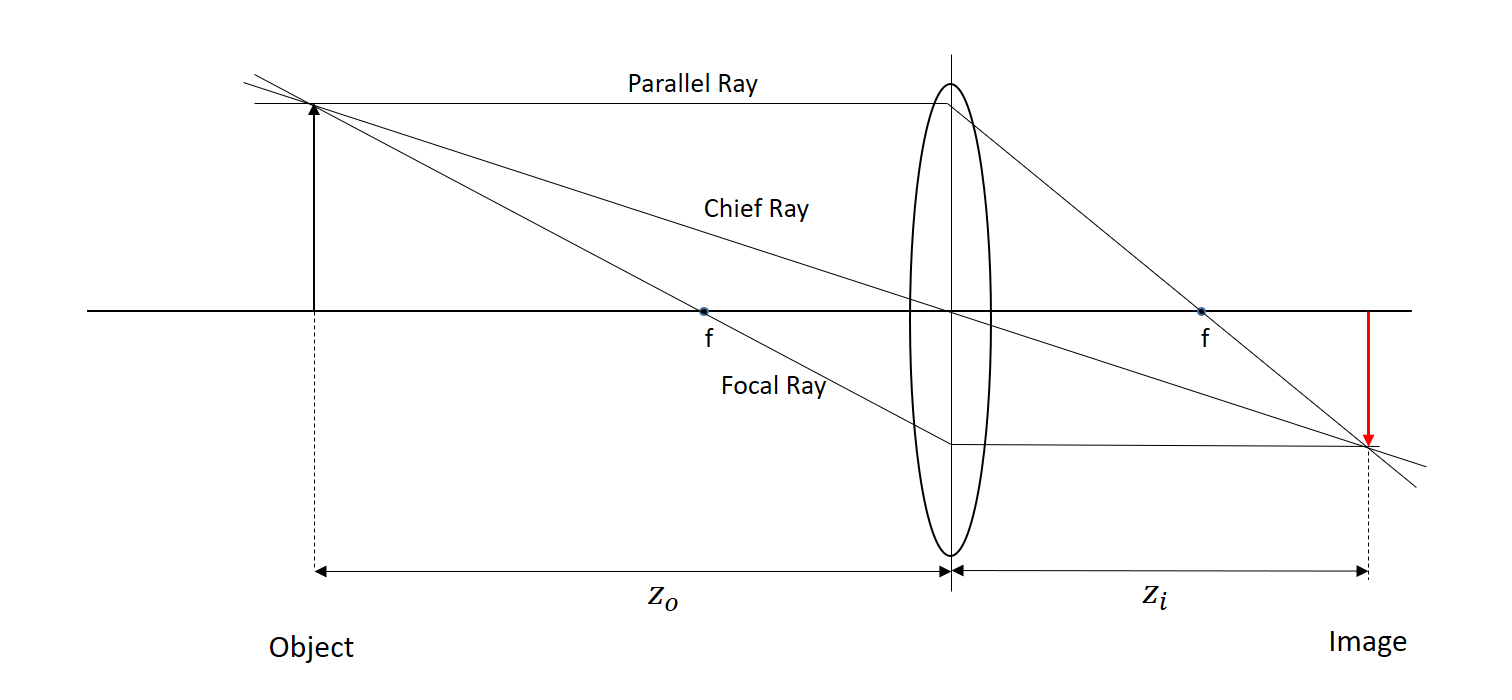
\includegraphics[width=5.0in]{chapters/chapter2/images/gauss.png}
  \caption{Gaussian Ray Tracing}
  \label{fig:ferrari}
\end{figure}

The distance from the object to the lens ($z_o$) and the distance from the image to the lens ($z_i$) are related by the following equation: 

$$\frac{1}{f} = \frac{1}{z_i} + \frac{1}{z_o}$$
 
\section{Myopia}
In a myopic or nearsighted eye, light rays converge in front of the retina. 

\begin{figure}[ht]
  \centering
  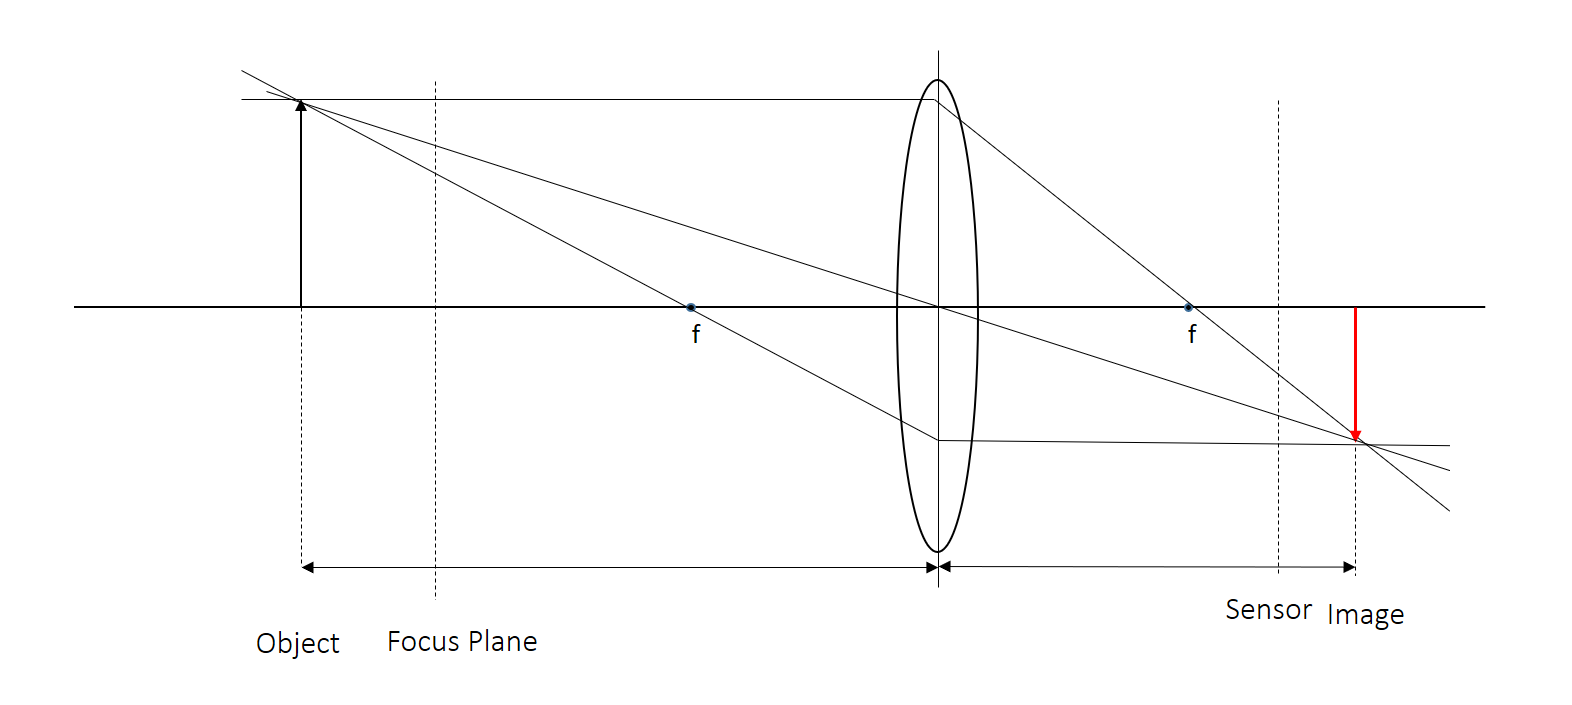
\includegraphics[width=5.0in]{chapters/chapter2/images/myopia.png}
  \caption{Myopia}
  \label{fig:ferrari}
\end{figure}

Myopia affects about 30 to 40 percent among adults in Europe and the United States, and up to 80 percent or higher in the Asian population, especially in China. In addition, incidence of myopia is increasing, from about 25 percent of Americans in the early 1970s to nearly 40 percent of the population today.

% Cite this: http://www.allaboutvision.com/parents/myopia-progression.htm

\section{Hyperopia}
In a hyperopic or farsighted eye, light rays converge behind the retina. 

\begin{figure}[ht]
  \centering
  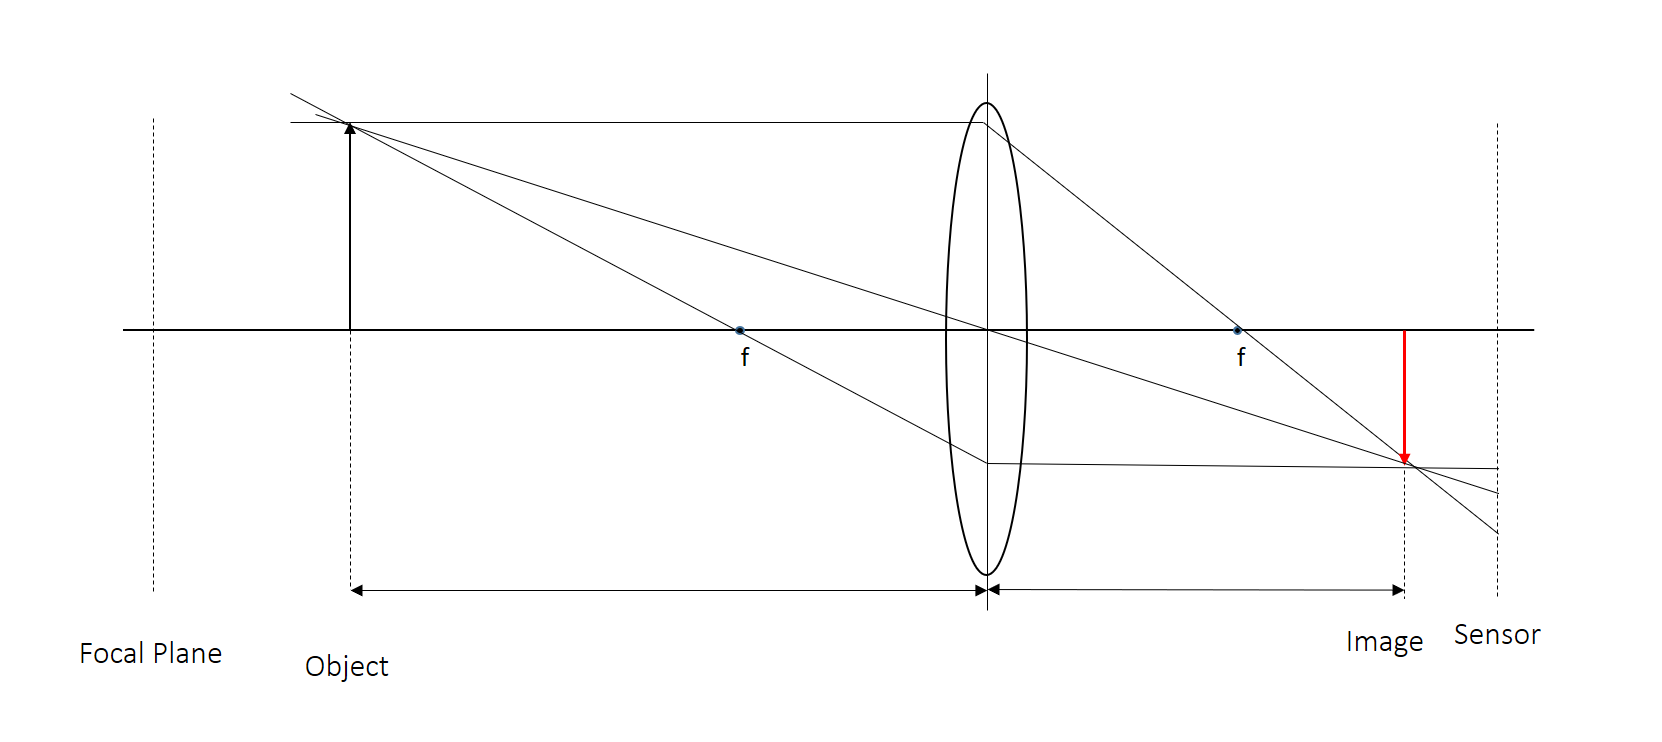
\includegraphics[width=5.0in]{chapters/chapter2/images/hyperopia.png}
  \caption{Hyperopia}
  \label{fig:ferrari}
\end{figure}

Hyperopia is a common condition that affects about ten percent of the adult population worldwide. 

% Cite this: http://www.drbishop.com/view/article_445.3conx

\section{Zernike Polynomials and Higher Order Aberrations}

We fit the wave aberrations with the Zernike polynomials, which are a set of shapes orthogonal to the unit disk used to measure the eye’s wavefront (Weisstein). The Zernike shapes are very similar to the usual aberrations that are found in a human eye. If we consider W(x,y) as the wavefront, then here is the equation that fits the Zernike polynomial:

$$W(x,y)= \sum_{i} c_i Z_i (x,y)$$

i represents the index of the coefficient c, and Z(x,y) is the associated polynomial equation. Here are the first six terms of the Zernike polynomial:

\begin{equation}
\begin{aligned}
W(x,y) ={} & c_0 \times 1 + c_1 \times 2 \times \rho \times sin(\theta) + c_2 \times 2 \times \rho \times cos(\theta) \\
           & + c_3 \times \sqrt{6} \rho^2 \times sin(2\theta) + c_4 \times \sqrt{3} \times (2 \times \rho^2 - 1) \\
           & + c_5 \times \sqrt{6} \times \rho^2 \times cos(2\theta) + ...
\end{aligned}
\end{equation}

\begin{figure}[ht]
  \centering
  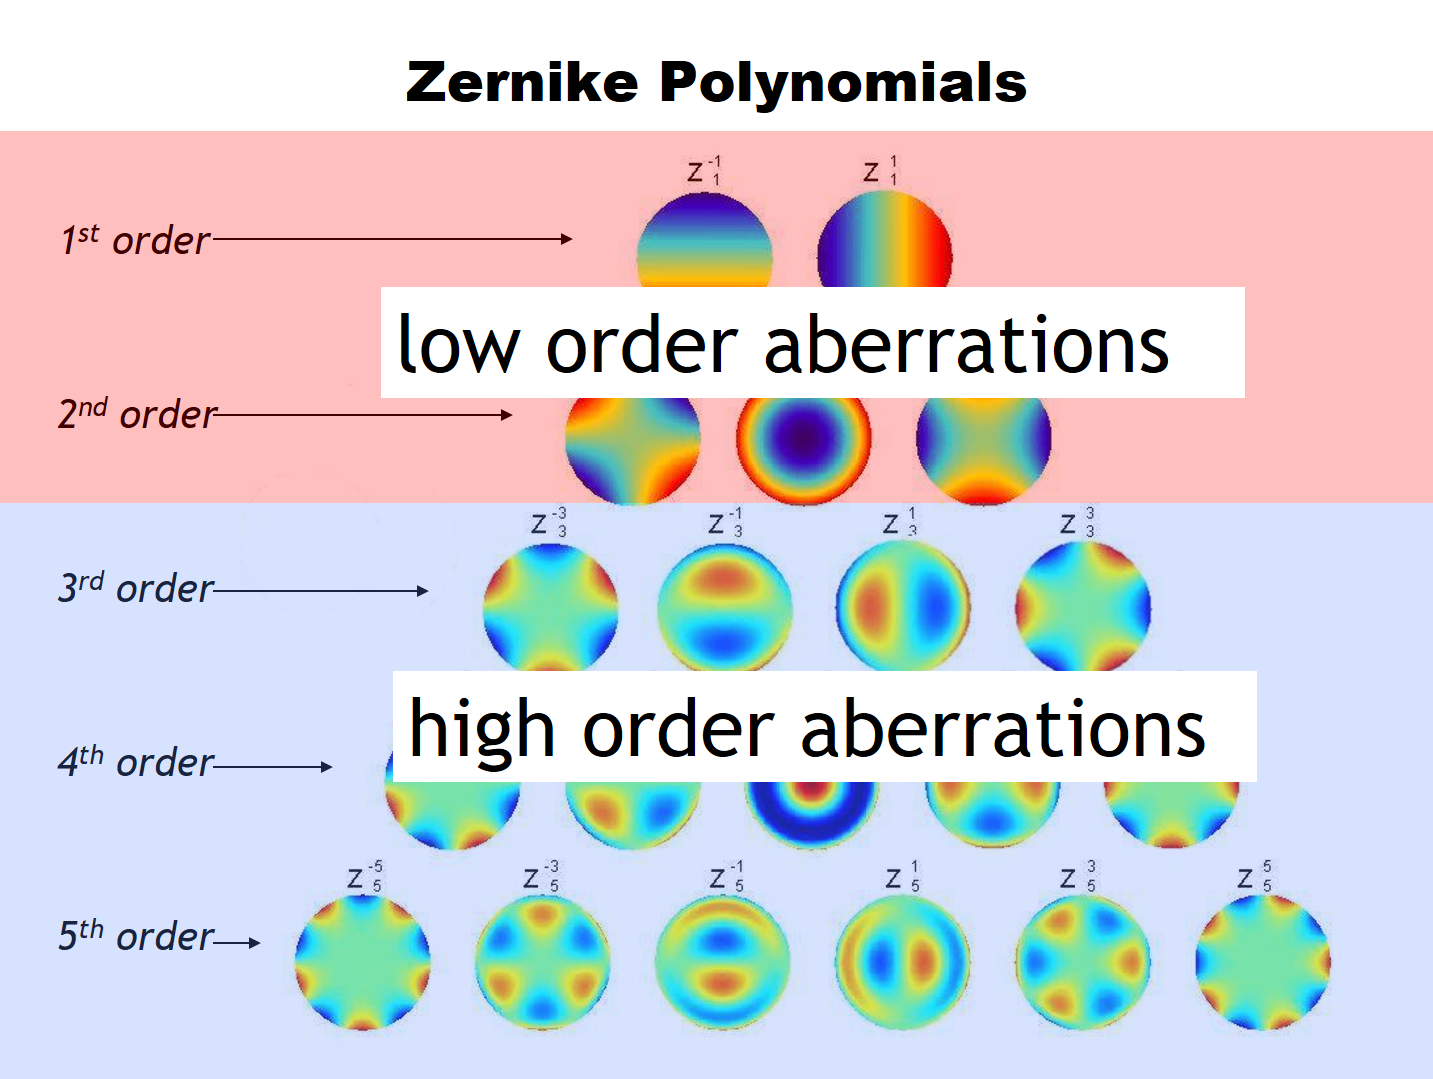
\includegraphics[width=5.0in]{chapters/chapter2/images/Zernike_polynomials.png}
  \caption{Hyperopia}
  \label{fig:ferrari}
\end{figure}

The first six Zernike polynomial terms measure lower order aberrations and the next sixty terms measure higher order aberrations. The names of lower order aberrations are tilt (terms one and two), astigmatism (terms three and five), and defocus (term four). Some examples of higher order aberrations are coma and trefoil (terms six through nine) and quatrefoil, secondary astigmatism, and spherical aberration (terms ten through fifteen). Lower order aberrations account for 90 percent of all decline in the quality of retinal images, while higher order aberrations are while the remaining 10 percent is a combination of the effects of higher order aberrations. Lower order aberrations are frequently treated with eyeglasses, which divert the direction of light rays so that they land squarely on the retina. However, higher order aberrations are much harder to treat with eyeglasses, but with the vision-correction display, a user can input the Zernike polynomial coefficients to manipulate the image on the screen.

% Cite this paper: http://www.scielo.br/pdf/rbof/v73n6/0034-7280-rbof-73-06-0358.pdf

% Question: Do I cite the PSF and wavefront map stuff?

% Do I mention circle of confusion?


% Cite Professor Austin's powerpoint slide

